\section{Introduction}
\label{sec:intro}

%
%%1. What is E-commerce shopping guide assistant?
An intelligent E-commerce online shopping guide assistant
is a comprehensive human-like system providing various services
such as pre-sale and after-sale inquiries, product recommendations,
and user complaints processing,
all of which seek to give the customers better shopping experience.
%%2. Dialog system and slot filling
The core of such assistant is a dialog system which 
has the ability to understand natural language utterances
from a user and then give natural language responses.
The architecture of a task-oriented dialog system
for online shopping guide assistant is illustrated in \figref{fig:dialog-system}.
%Besides modules of dialog management (DM) and 
%natural language generation (NLG),
%the very fist step of a dialog system is 
Natural Language Understanding (NLU), which aims to 
interpret the semantic meanings conveyed by input utterances
is a main component in task-oriented dialog systems. 
Slot filling is a subproblem in NLU, which identifies
the properties and their values about the task to be performed in
the dialog.

\begin{figure}[h]
	\centering
	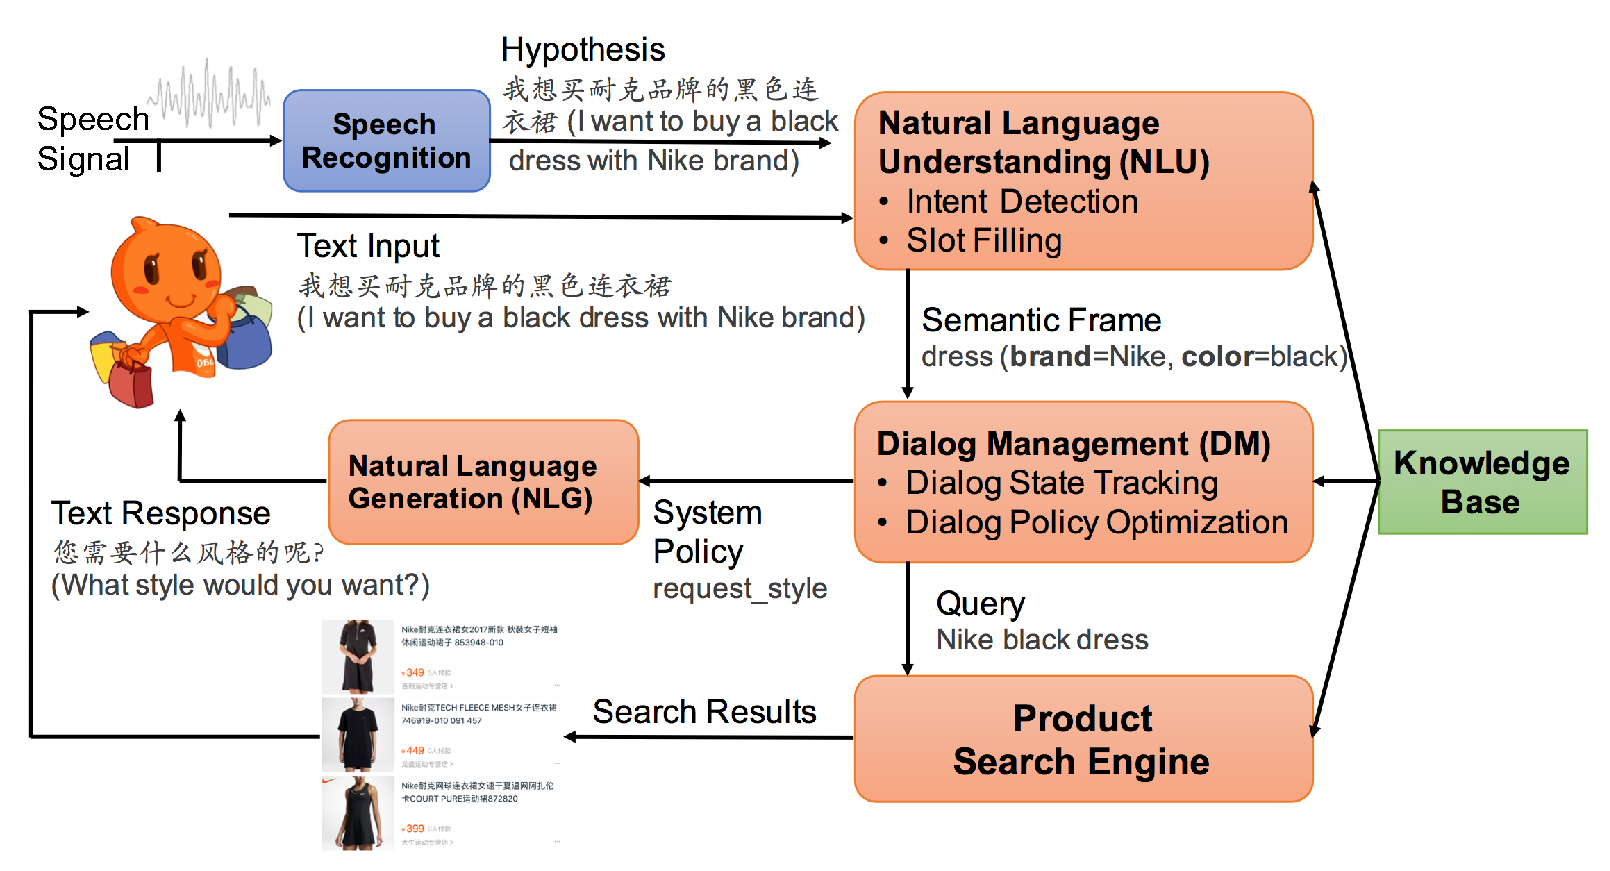
\epsfig{file=figures/dialog_system.eps, width=1.0\columnwidth}
	\caption{Pipeline framework of task-oriented dialog system for shopping guide assistant.}
	\label{fig:dialog-system}
	\vspace{-10pt}
\end{figure}

Slot filling extracts semantic constituents
by using the words of input text to fill in pre-defined slots in 
a semantic frame \cite{mesnil2015using}.
It can be regarded as sequence labeling task,
which assigns an appropriate semantic label to each word in
the given input utterance. 
In the case of E-commerce shopping, 
there are three named entity types including 
\emph{Category}, \emph{Property Key} and \emph{Property Value}.
We show a real example in \tabref{tab:slot-filling-demo}
with In/Out/Begin(IOB) scheme.
In the named entity level,
``连衣裙''\emph{(dress)} is a Category (\textbf{B-CG}/\textbf{I-CG}),
while ``品牌''\emph{(brand)} is labeled as Property Key
(\textbf{B-PK}/\textbf{I-PK}),
which is the name of one product property.
``耐克''\emph{(Nike)} and ``黑色''\emph{(black)} are labeled as Property Value
(\textbf{B-PV}/\textbf{I-PV}) since they are concrete property values.
However, labeling as Property Value is not good enough for NLU.
Thus, in Slot Filling level, 
we further label ``耐克''\emph{(Nike)} as Brand Property (\textbf{B-Brand}/\textbf{I-Brand}), 
and ``黑色''\emph{(black)} as 
Color Property (\textbf{B-Color}/\textbf{I-Color}).
In the meantime, 
other words in the example utterance that carry no semantic meaning are assigned \textbf{O} label.
\begin{table*}[h]
	\centering
	\scriptsize
	\begin{tabular}{c|c|c|c|c|c|c|c|c|c|c|c|c|c}
		\toprule
		\multirow{2}{*}{Utterance} & 我 & 想 & 买 & 耐 & 克 & 品 & 牌 & 的 & 黑 & 色 & 连 & 衣 & 裙 \\
		\cmidrule{2-14}
		& \em{I} & \em{want} & \em{buy} & \multicolumn{2}{c|}{\em{Nike}} & \multicolumn{2}{c|}{\em{brand}} & $\backslash$  & \multicolumn{2}{c|}{\em{black}} & \multicolumn{3}{c}{\em{dress}} \\
		\midrule
		Slot Label & \textbf{O} & \textbf{O} & \textbf{O} & \textbf{B-Brand} & \textbf{I-Brand} & \textbf{B-PK} & \textbf{I-PK} & \textbf{O} & \textbf{B-Color} & \textbf{I-Color} & \textbf{B-CG} & \textbf{I-CG} & \textbf{I-CG} \\
		\midrule
		Named Entity Label & \textbf{O} & \textbf{O} & \textbf{O} & \textbf{B-PV} & \textbf{I-PV} & \textbf{B-PK} & \textbf{I-PK} & \textbf{O} & \textbf{B-PV} & \textbf{I-PV} & \textbf{B-CG} & \textbf{I-CG} & \textbf{I-CG} \\
		\midrule
		Segment Label & \textbf{O} & \textbf{O} & \textbf{O} & \textbf{B} & \textbf{I} & \textbf{B} & \textbf{I} & \textbf{O} & \textbf{B} & \textbf{I} & \textbf{B} & \textbf{I} & \textbf{I} \\
		\bottomrule
	\end{tabular}
	\caption{A real example of slot filling in online shopping scenario.}
	\label{tab:slot-filling-demo}
	\vspace{-10pt}
\end{table*}

State-of-the-art sequence labeling models are typically based on 
BiLSTM and CRF \cite{huang2015bidirectional,reimers2017optimal}
and evaluated on a commonly used standard dataset ATIS \cite{price1990evaluation} in slot filling area.
This dataset is in the domain of airline travel in America and
\tabref{tab:slot-filling-demo-atis} shows an example utterance.
However,
the vocabulary size of ATIS is too small (only 572)
and slot labels are not diverse enough
since airline travel is a relatively small and specific domain,
such that recent deep learning models can achieved very high F1 scores
(nearly 0.96).
\begin{table}[h]
	\centering
	\scriptsize
	\begin{tabular}{c|c}
		\toprule
		Utterance & flights $|$ from $|$ Dallas $|$ to $|$ New York \\
		\midrule
		Slot Label & \makecell{\textbf{O} $|$ \textbf{O} $|$ \textbf{B-fromloc.city\_name} $|$ \textbf{O} $|$ \textbf{B-toloc.city\_name} $|$ \\ \textbf{I-toloc.city\_name}}  \\
		\bottomrule
	\end{tabular}
	\caption{An example utterance from the ATIS dataset.}
	\label{tab:slot-filling-demo-atis}
	\vspace{-10pt}
\end{table}

Compared to ATIS, our E-commerce shopping guide assistant dataset is 
more complex.~\footnote{This dataset is available at \url{http://Anonymized.for.blind.review}.}
This dataset comes from a real world application and the
semantic slots are more diverse and informal than ATIS, 
which increases the difficulty for the task.
%For example, there are 26 semantic labels in the Dress category,
%which describe different properties for a dress such as color, brand and style, while most semantic labels of ATIS 
%are related to only time and location.
For example, to describe different properties for a product for purpose of utterance understanding and query rewrite,
we should define large amount of informative slot labels such as color, brand, style, season, gender and so on.
While most semantic labels of ATIS are related to only time and location.
On the other hand, the spoken E-commerce Chinese language is more complex and enriched expression makes it harder to understand.
For example, ``红色'' and ``红'' both mean red, ``品牌'' and ``牌子'' both mean brand, ``耐克'' and ``Nike'' and ``Niky'' all mean Nike.
While in ATIS, expression can be simpler, and most expressions are standard locations or time.

Besides, Chinese language, like many other Asian languages, are not
word segmented by nature, and word segmentation is a difficult
first step in many NLP tasks.
Without proper word segmentation, sequence labeling becomes very challenging
as the errors from segmentation will propagate.
On the other hand, more than 97\% of the chunks in ATIS data 
have only one or two words,
in which segment (or chunking) may not be a serious problem.
%Due to these reasons,
%if we simply apply basic sequence labeling models 
%to Chinese E-commerce dataset,
%the model even can not segment the sequence correctly.
%Then the errors will propagate and the resulting slot labels will incorrect.

%4. How Deep Cascade Multi-task learning works and the performance?
%In this paper, we employ the idea of multi-task learning
%to tackle slot filling task in Chinese E-commerce.
In this paper, we are the first to employ multi-task sequence labeling model
to tackle slot filling in a novel Chinese E-commerce dialog system.
We divide the slot filling task into two lower-level tasks: 
{\em named entity tagging} and {\em segment tagging}.
Example labels of these two tasks 
are shown in the bottom two rows of \tabref{tab:slot-filling-demo}.
Segment tagging and named entity tagging can be regarded as 
syntactic labeling, 
while slot filling is more like semantic labeling.
Once we know the syntactic structure of an input sentence,
filling the semantic labels becomes easier.
Compared to directly attacking slot filling,
these two low-level tasks are much easier to solve
due to fewer labels.
To this end, we propose a Deep Cascade Multi-task Learning model,
and co-train three tasks in the same framework
with a goal of optimizing the target slot filling task.

%5. Contribution and Conclusion.
%\xusheng{Need this part? or add something else}
The contributions of this paper are summarized below:
\begin{itemize}
	\itemsep0em
	\item This is the first attempt to attack the real-world problem of 
	slot filling for Chinese E-commerce online shopping guide assistant system (\secref{sec:problem}).
	\item We are the first to propose a Chinese dialog spoken language dataset ECSGA (\secref{sec:data}).
	Its domain is much different from common ATIS dataset and it has much more data.
	We believe this dataset will contribute more to the future research of dialog natural language understanding.
	\item We present a novel deep multi-task sequence labeling model with cascading and 
	residual connection to solve slot filling problem
	(\secref{sec:dcmtl}), and the results 
	show the model outperforms 
	several strong baseline methods 
	by a substantial margin of $14.6\%$ on $F1$ score (\secref{sec:eval}). 
\end{itemize}
